\chapter{State Estimation}
\label{ch:estimation}
*** Talk about quantifying the performance of the ACS Kalman filter \cite{Sights06}. Discuss training of the covariance matrices. Show the position estimation using the original covariance matrices and the ones found from training. If I get to identifying bias and/or drift in the IMU put that here as well. ***

The Space and Naval Warfare Systems Center, San Diego (SSC-SD) robotics group has developed the Autonomous Capabilities Suite (ACS) which incorporates many different technologies into a single software package that can be run on a wide variety of robots and is able to easily accomodate different payload and sensor suites \cite{Sights06}. One of the ACS libraries is the adaptive extended Kalman filter which is used on the EOD robots for state estimation and is the main method used for answering the question ``Where am I?''. The idea behind the Kalman filter is relatively straightforward. The robot has some basic idea of where it is in the world but there is some uncertainty involved in that estimate due to different measurement accuracies from multiple sensors that measure the same state, noise in the individual sensor measurements and an imperfect model of how the robot moves through the world. Some of the uncertainty of the model can be explained by the fact that not all of the necessary measurements are being carried out and the states can be unobservable. *** Say more here about noise/uncertainty. ***

An example is a robot driving in a straight line where the left track may be moving on a flat surface while the right track is moving on an uneven surface as in Figure \ref{fig:topography}. The wheel encoders that measure how far each track is moving will report that the right track is traveling a greater distance than the left track which could mean that the robot is turning counter-clockwise or that the robot tracks are moving over different surface types. At the same time the robot will be getting measurements about its heading from both the IMU and GPS sensors that will have some noise as well. In this example both the IMU and GPS sensors would likely say that the robot is traveling in a straight line on average (as long as the controller is performing adequately). The job of the Kalman filter is to determine how much each sensor should be trusted when trying to determine where the robot really is in the world and how fast it is moving. This is accomplished by looking at each of the noise parameters for both the system model and the measurements as being zero mean, white noise, uncorrelated, Gaussian variables ... *** Clean up this language. Consider putting it in a different section like \S\ref{sec:duals}. ***

\begin{figure}[ht!]
	\centering
	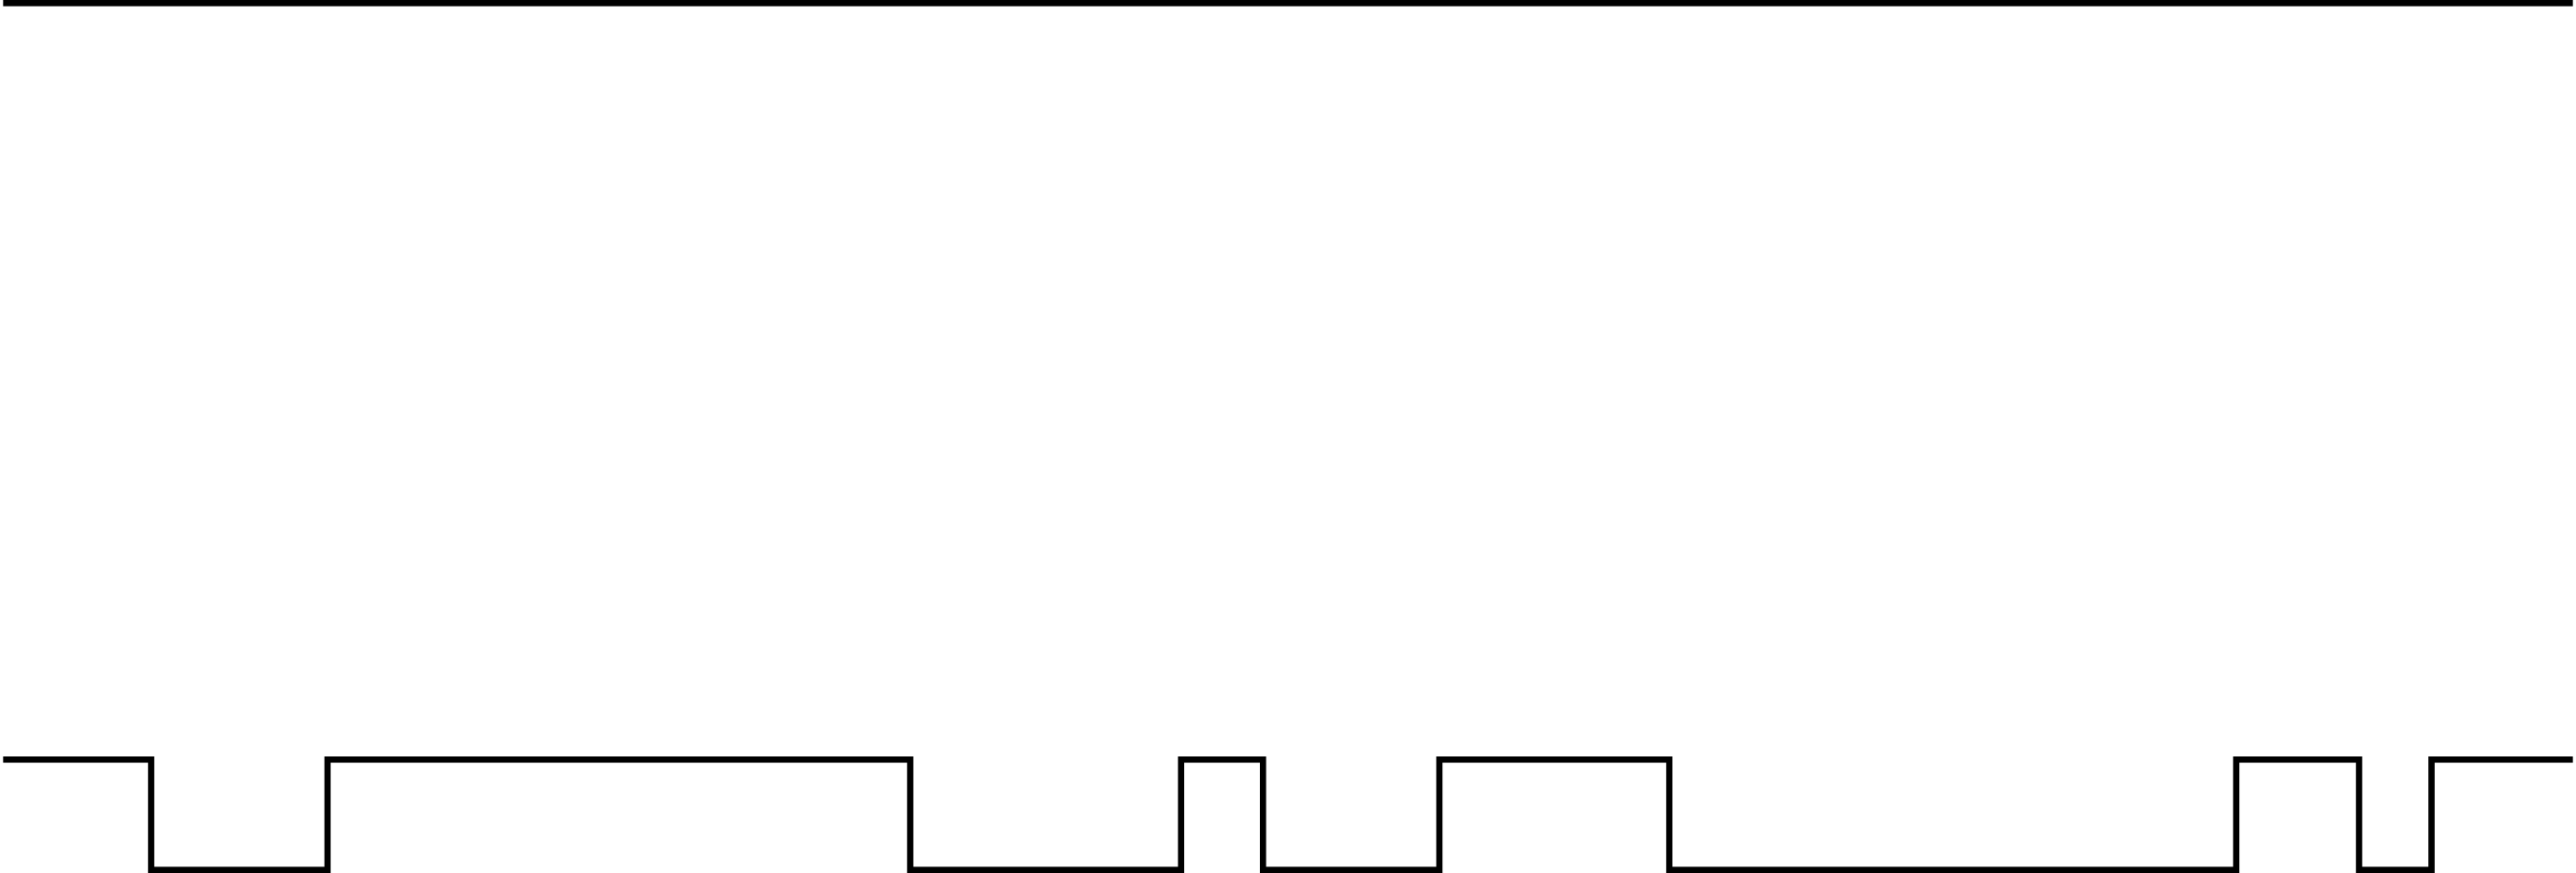
\includegraphics[width=.5\textwidth]{images/topography}
	\caption{Different topographies for the left track and the right track when the ground is smooth on the left side and bumpy on the right side. The top line is for the left track and the bottom line is for the right track.}
	\label{fig:topography}
\end{figure}

\section{State Space Models}
\label{sec:statespacemodels}
Kalman filters and control systems (see Chapter \ref{ch:controls}) use the idea of a multi-dimensional state space to encapsulate all of the relevant information that is known about a system. In the case of robots the dynamics are typically captured by position, orientation, linear and angular velocities, acceleration and sometimes jerk. The general equations to describe the state space of a system are

\begin{align}
\label{eq:statespace}
\begin{split}
\dot{x} &= f(x,u,t) \\
\dot{y} &= h(x,t)
\end{split}
\end{align}

The state variables are given in vector form by $x$ and the sensor measurements are contained in the vector $y$. The state space equations are a means of representing how the state and measurements of a system change through time based on the initial state of the system and the inputs, $u$, to the system which allows the trajectory (or motion through time) and the effect of the trajectory on the measurements to be calculated using compact notation. The inputs are assumed to include any external forces applied to the system as well as actuation provided by the system itself.

\section{The Kalman Filter}
\label{sec:kalmanfilter}
The ACS Kalman filter is typical of all Kalman filters in that it consists of a prediction update step and a measurement update step where the prediction update is run as fast as possible and the measurement update is run whenever new sensor data becomes available as in Figure \ref{fig:kf}. The prediction update step uses a model of the system dynamics and a measurement of elapsed time to determine where the system is in the world and will inevitably have errors due to effects that are not captured by the model, especially when the system dynamics are linearized. The measurement update step is basically a feedback step to help correct for errors in the system model using sensors to provide current data \cite{Kelly_1994_338}.

\begin{figure}[ht!]
	\centering
	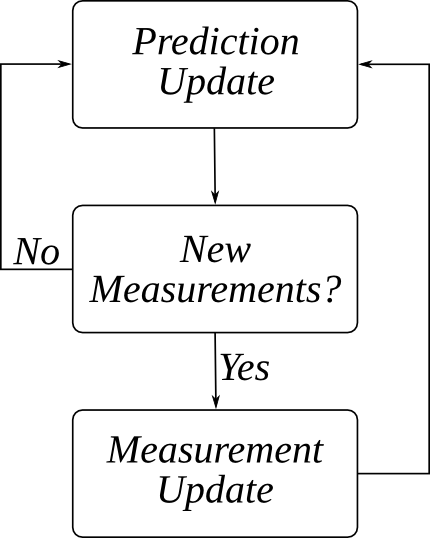
\includegraphics[width=.4\textwidth]{images/kf}
	\caption{The Kalman filter algorithm.}
	\label{fig:kf}
\end{figure}

The Kalman filters that run on the small UGVs used in these experiments run on digital computers and are necessarily discretized forms because of the nature of computers. From \cite{Kelly_1994_338}, \cite{Simon06OptimalEstimation} the discretized versions of (\ref{eq:statespace}) mean that the state space equations are

\begin{align}
\label{eq:kfstatemodel}
\begin{split}
x_{k+1} &= F_kx_k + \Gamma_kw_k \\
y_k &= H_kx_k + v_k
\end{split}
\end{align}
where $F_k$ is the state transition matrix relating the state at time $k+1$ to time $k$ in the absence of inputs or noise, $\Gamma_k$ is the noise distribution matrix which translates the input vector $w_k$ into the coordinates of the state, $H_k$ is the measurement matrix which relates the measurements to the state vector and $v_k$ is the sensor measurement noise.

The prediction update step marches the system dynamics forward in time using the equations

\begin{align}
\label{eq:kfpredictionupdate}
\begin{split}
\hat{x}_{k+1}^- &= \Phi_k\hat{x}_k^+ \\
P_{k+1}^- &= F_kP_k^+F_k^T + \Gamma_kQ_k\Gamma_k^T
\end{split}
\end{align}
and the measurement update step provides feedback from sensor data using the equations

\begin{align}
\label{eq:kfmeasurementupdate}
\begin{split}
K_k &= P_k^-H_k^T\left[H_kP_k^-H_k^T + R_k\right]^{-1} \\
\hat{x}_k^+ &= \hat{x}_k^- + K_k\left[y_k - H_k\hat{x}_k^-\right] \\
P_k^+ &= \left[I - K_kH_k\right]P_k^-
\end{split}
\end{align}

The prediction update step relies on knowing $\Phi_k$, $\Gamma_k$ and the disturbance covariance matrix, $Q_k$, while the measurement update step needs to know $H_k$ and the measurement covariance matrix, $R_k$. Using (\ref{eq:kfpredictionupdate}) and (\ref{eq:kfmeasurementupdate}) an estimate of the state of the robot can be obtained at any time for use by the controls algorithms.

\subsection{Extended Kalman Filter}
\label{sec:extendedkf}
The basic Kalman filter makes the assumption that both the system model contained in $F_k$ and the measurement model in $H_k$ are linear. The extended Kalman filter (EKF) allows for nonlinear models to be used for $F_k$, $H_k$ or both by linearizing the models around the state estimate. To linearize the models the Jacobian, or matrix of partial derivatives, is taken about the estimated state.

The state vector used in the ACS EKF follows that found in \cite{Kelly_1994_338}, \cite{Kelly_1994_333} which avoids issues of non-observability by using the principal motion assumption where the state variables are

\begin{align*}
x_k = \left[\begin{array}{c c c c c c c c} x & y & z & v & \theta & \phi & \psi & \omega \end{array}\right]^T
\end{align*}
In this vector $x$, $y$ and $z$ are positions, $v$ is velocity, $\theta$, $\phi$ and $\psi$ are Euler angles for pitch, roll and yaw, and $\omega$ is angular velocity as shown in Figure \ref{fig:robotaxes}.

\begin{figure}[ht!]
	\centering
	\subfloat[Urbot.]{
		\label{fig:urbotaxes}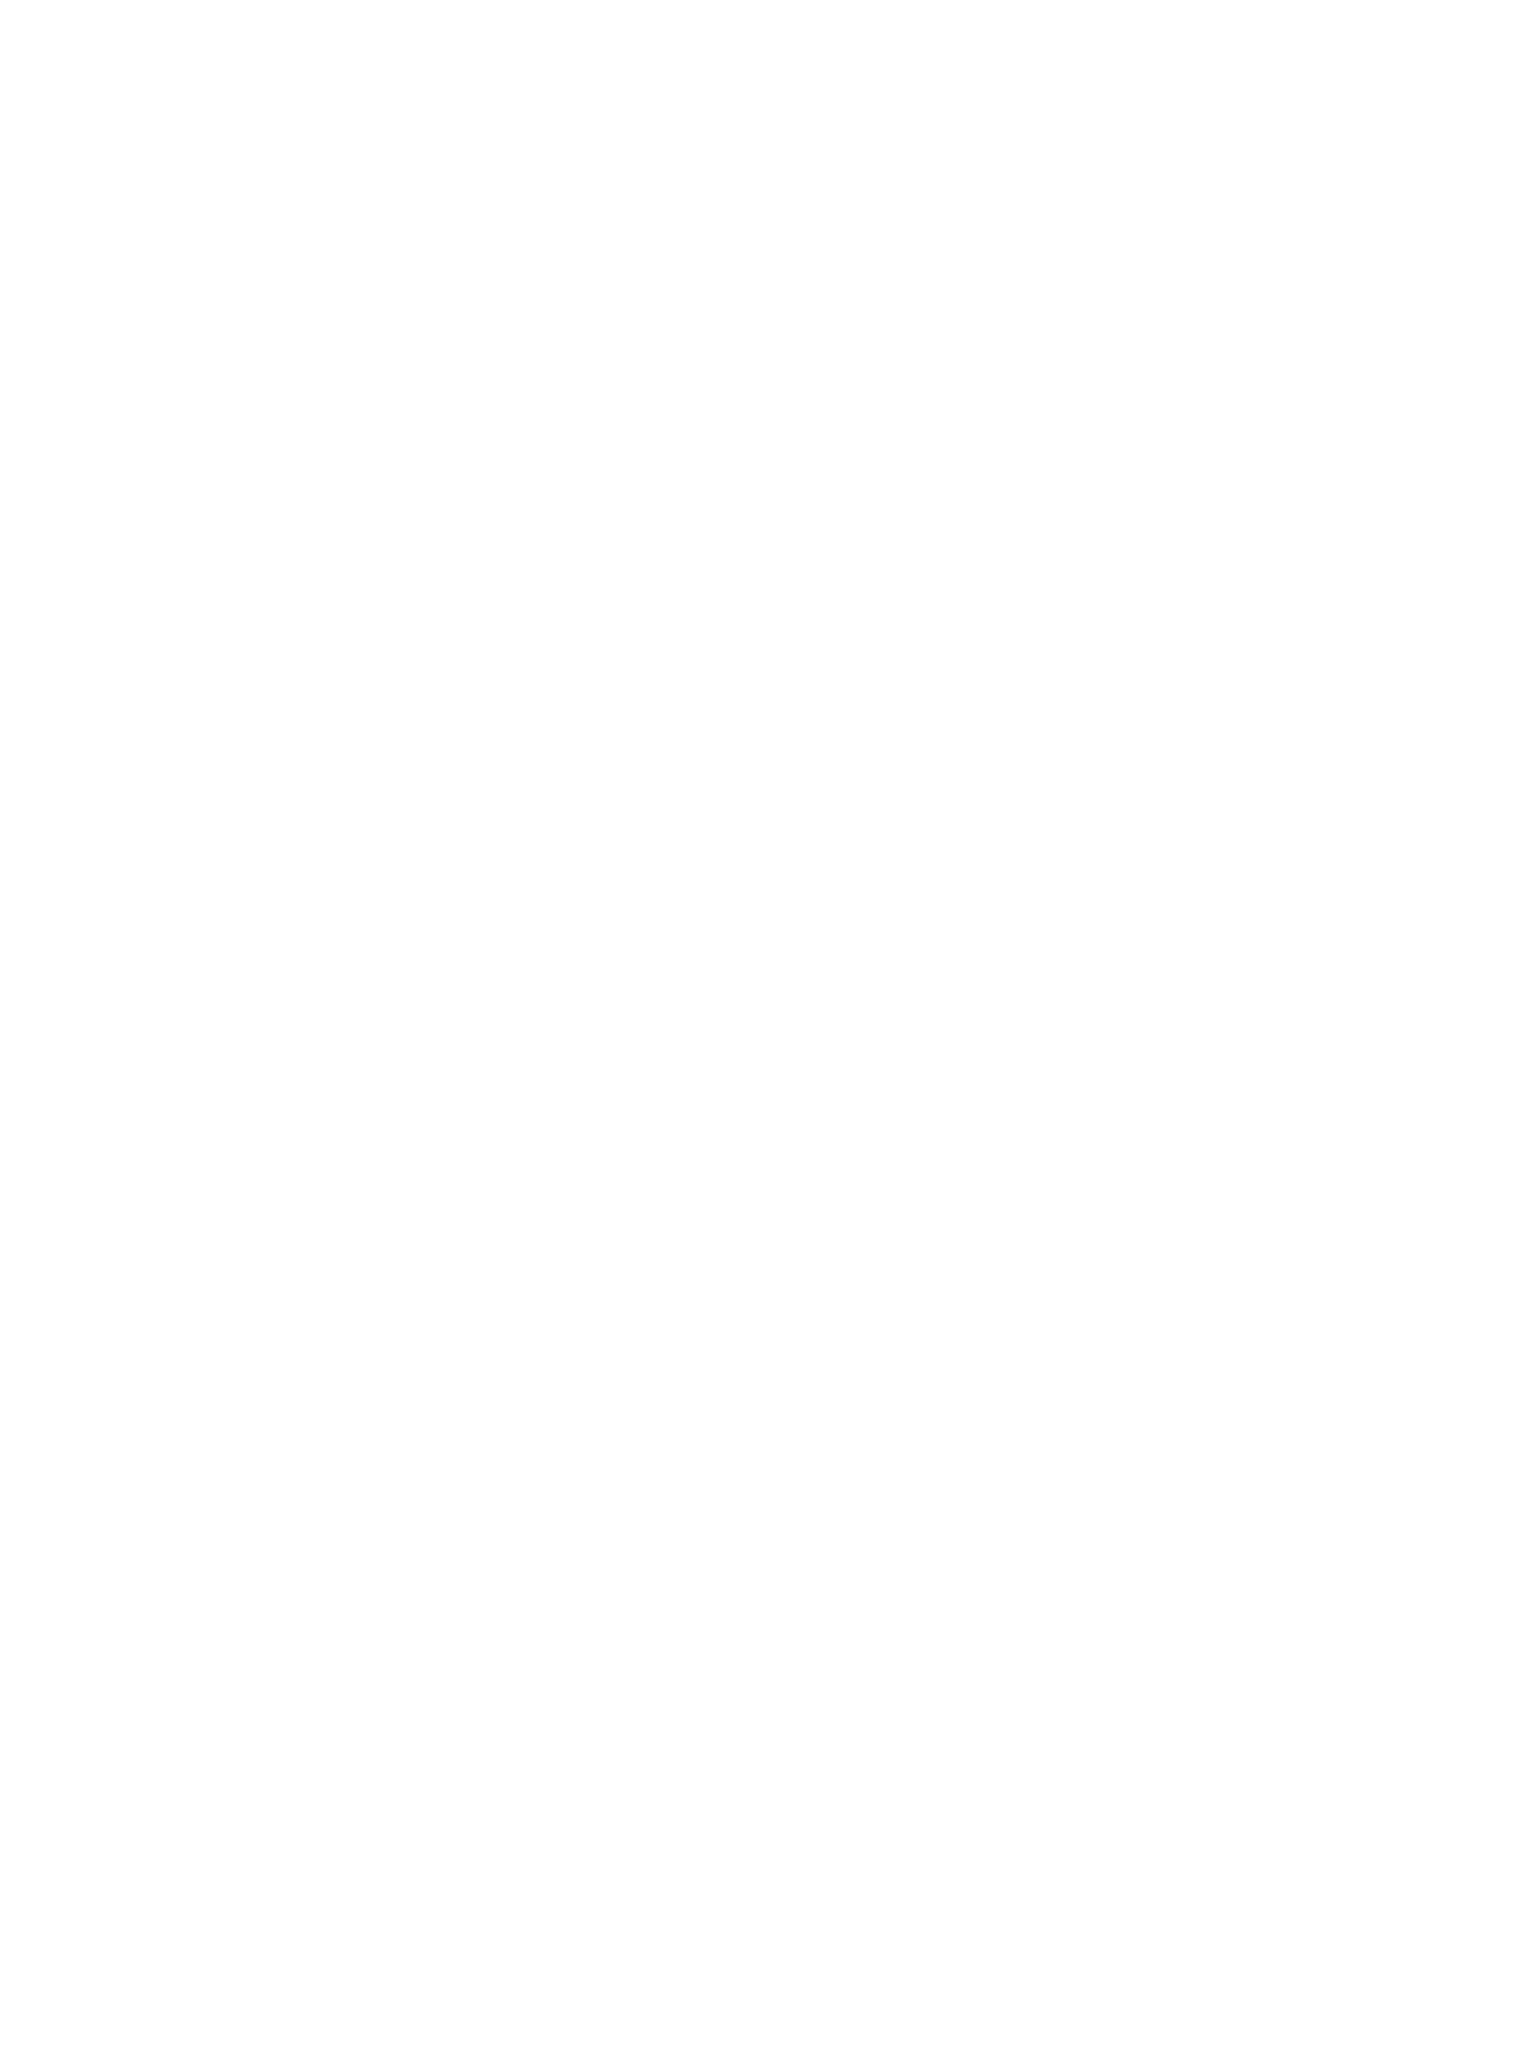
\includegraphics[width=.45\textwidth]{images/urbotaxes}
	} \qquad
	\subfloat[PackBot.]{
		\label{fig:pbaxes}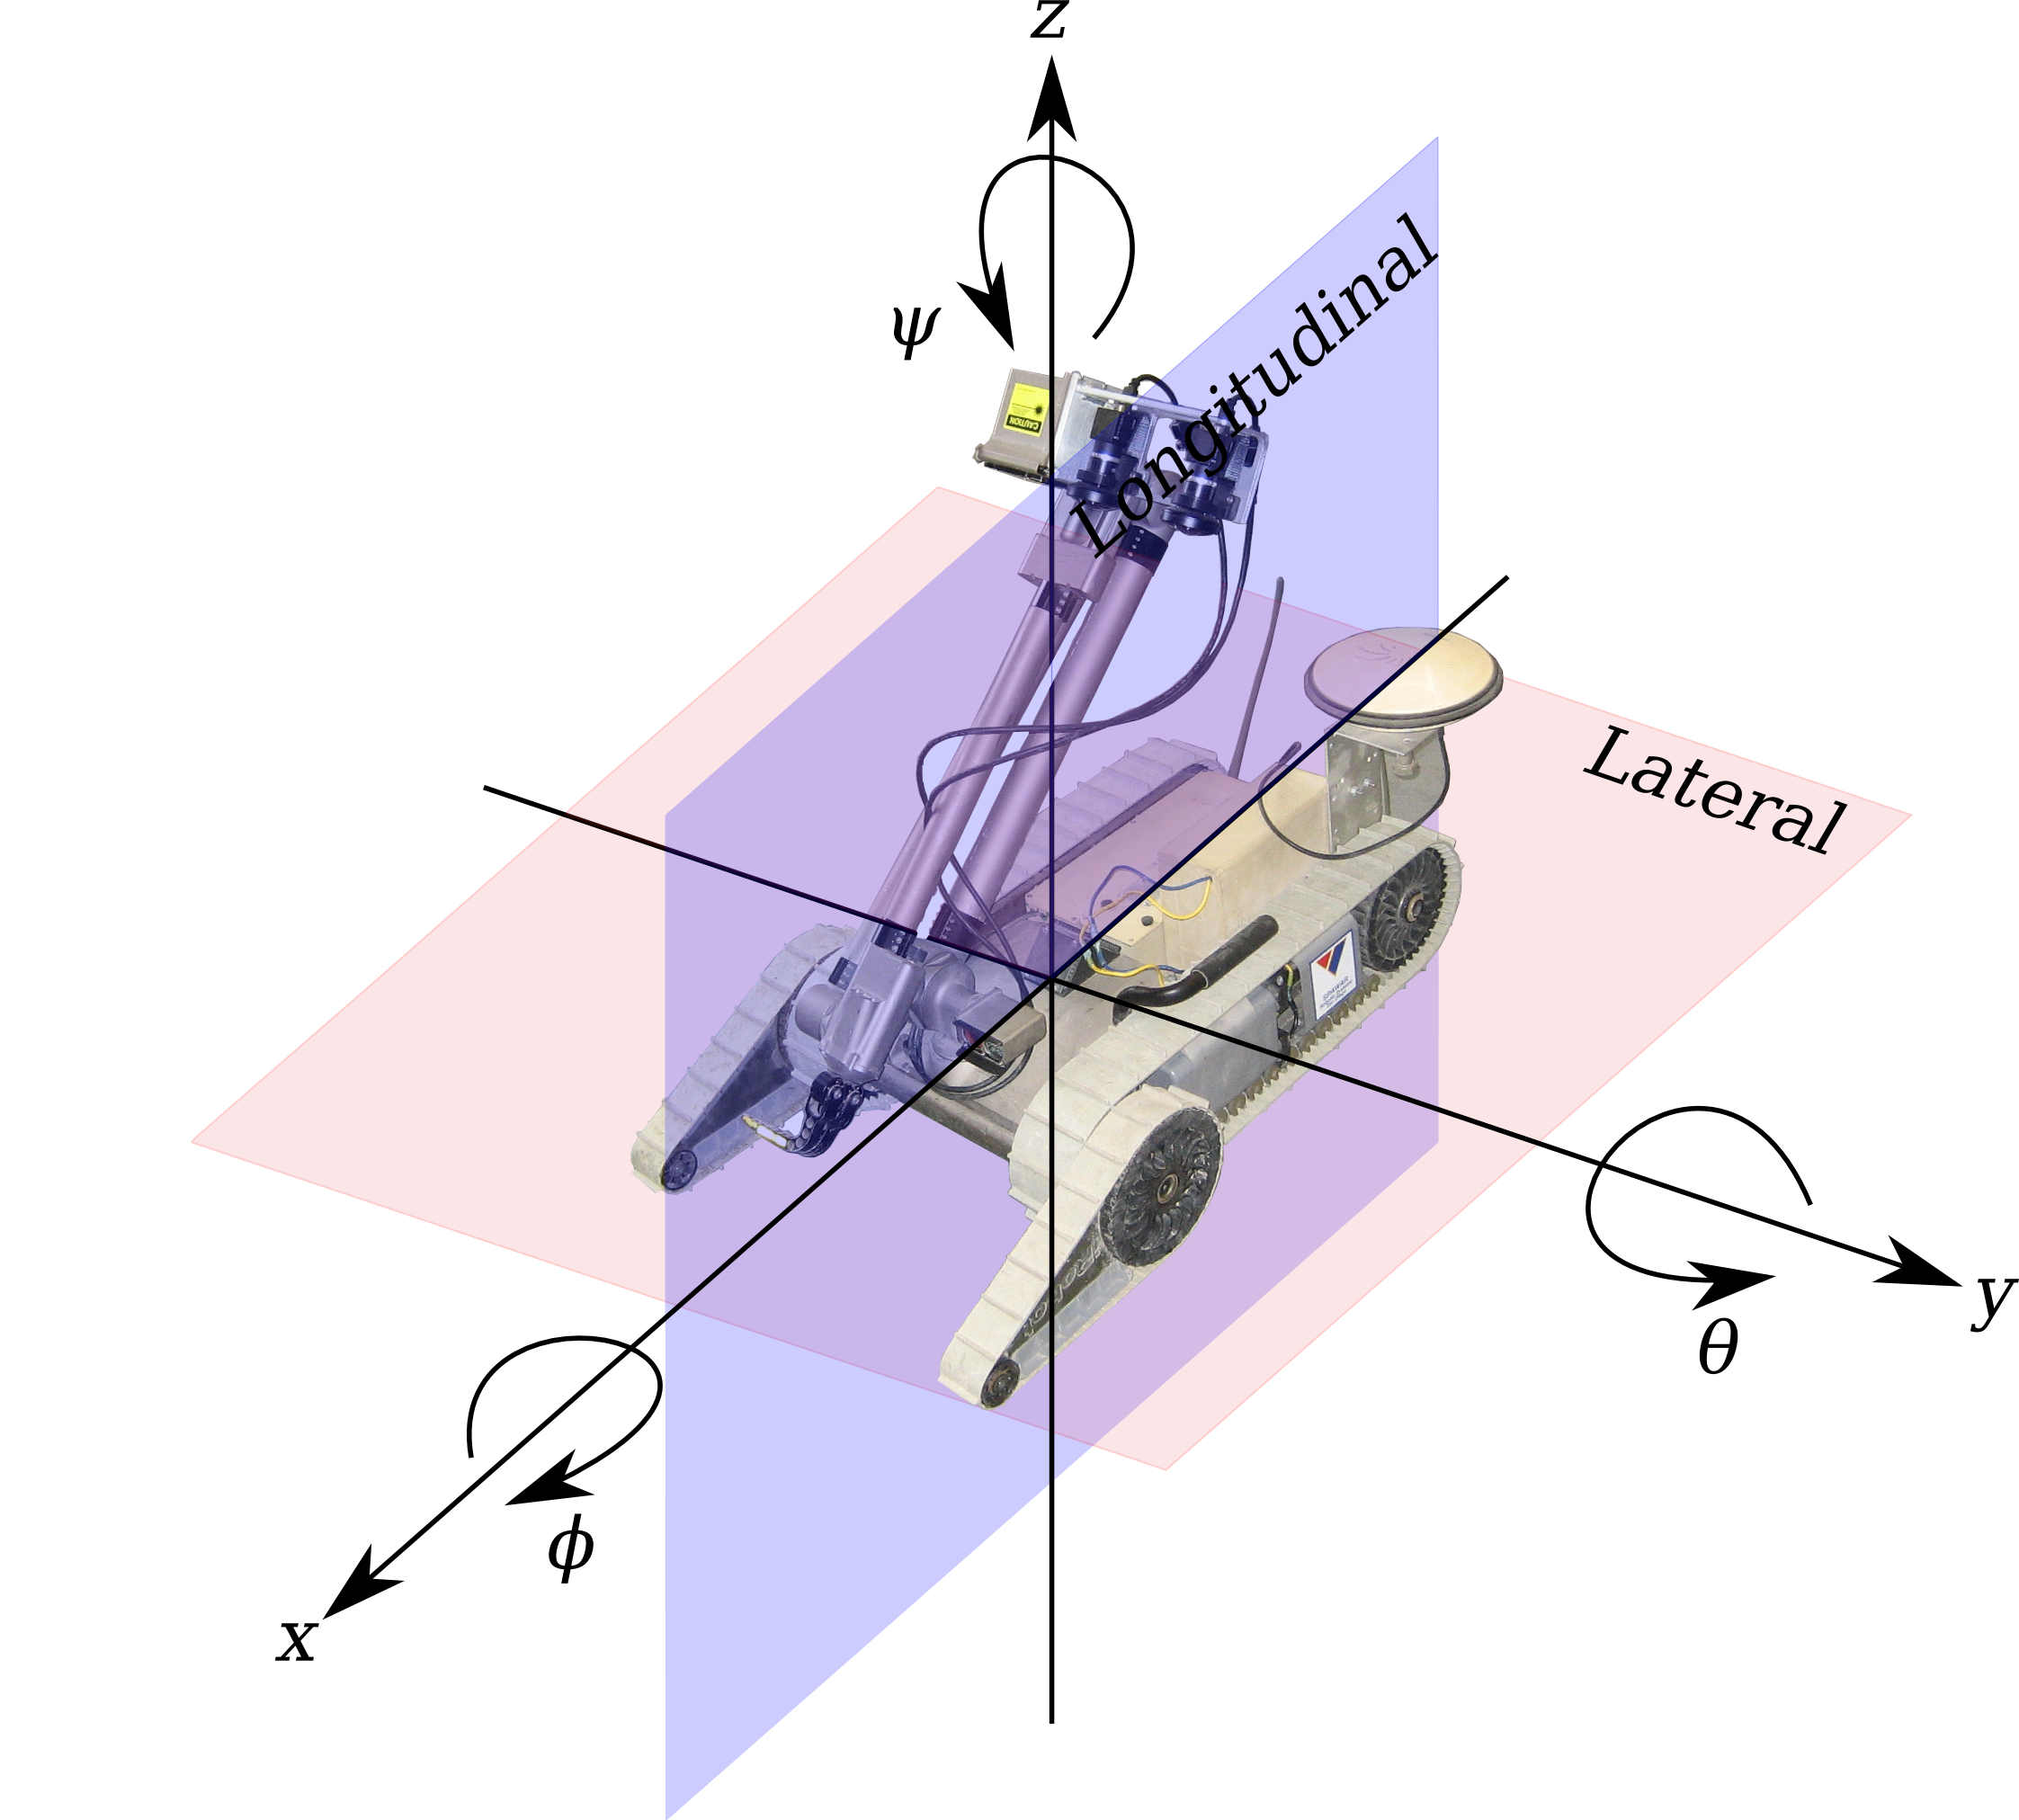
\includegraphics[width=.45\textwidth]{images/packbotaxes}
	}
	\caption{Robots used in experiments with axes for position and orientation shown..}
	\label{fig:robotaxes}
\end{figure}

The state transition matrix is

\begin{align}
\label{eq:kfF}
F = \left[\begin{array}{c c c c c c c c}
0 & 0 & 0 & F_{1,4} & F_{1,5} & 0 & F_{1,7} & 0 \\
0 & 0 & 0 & F_{2,4} & F_{2,5} & 0 & F_{2,7} & 0 \\
0 & 0 & 0 & F_{3,4} & F_{3,5} & 0 & 0 & 0 \\
0 & 0 & 0 & 0 & 0 & 0 & 0 & 0 \\
0 & 0 & 0 & 0 & 0 & F_{5,6} & 0 & F_{5,8} \\
0 & 0 & 0 & 0 & F_{6,5} & F_{6,6} & 0 & F_{6,8} \\
0 & 0 & 0 & 0 & F_{7,5} & F_{7,6} & 0 & F_{7,8} \\
0 & 0 & 0 & 0 & 0 & 0 & 0 & 0
\end{array}\right]
\end{align}
where the elements of $F$ are

\begin{align*}
\begin{split}
F_{1,4} &= \cos(\psi)*\cos(\theta)
\end{split}
\begin{split}
F_{1,5} = -v*\cos(\psi)*\sin(\theta)
\end{split} \\
\begin{split}
F_{1,7} &= -v*\sin(\psi)*\cos(\theta)
\end{split}
\begin{split}
F_{2,4} = \sin(\psi)*\cos(\theta) \\
\end{split} \\
\begin{split}
F_{2,5} &= -v*\sin(\psi)*\sin(\theta)
\end{split}
\begin{split}
F_{2,7} = v*\cos(\psi)*\cos(\theta) \\
\end{split} \\
\begin{split}
F_{3,4} &= -\sin(\theta)
\end{split}
\begin{split}
F_{3,5} = -v*\cos(\theta) \\
\end{split} \\
\begin{split}
F_{5,6} &= -\omega *\cos(\phi)
\end{split}
\begin{split}
F_{5,8} = -\sin(\phi) \\
\end{split} \\
\begin{split}
F_{6,5} &= \omega *\cos(\phi)/\cos^2(\theta)
\end{split}
\begin{split}
F_{6,6} = \omega *\tan(\theta)*\sin(\phi) \\
\end{split} \\
\begin{split}
F_{6,8} &= \tan(\theta)*\cos(\phi)
\end{split}
\begin{split}
F_{7,5} = \omega *\sin(\theta)*\cos(\phi)/\cos^2(\theta) \\
\end{split} \\
\begin{split}
F_{7,6} &= -\omega *\sin(\phi)/\cos(\theta)
\end{split}
\begin{split}
F_{7,8} = \cos(\phi)/\cos(\theta)
\end{split}
\end{align*}
This gives the nonlinear state equations as

\begin{align*}
x_{k+1} &= \cos(\psi_k)*\cos(\theta_k)*v_k - v_k*\cos(\psi_k)*\sin(\theta_k)*\theta_k \\
&\qquad- v_k*\sin(\psi_k)*\cos(\theta_k)*\psi_k \\
y_{k+1} &= \sin(\psi_k)*\cos(\theta_k)*v_k - v_k*\sin(\psi_k)*\sin(\theta_k)*\theta_k \\
&\qquad+ v_k*\cos(\psi_k)*\cos(\theta_k)*\psi_k \\
z_{k+1} &= -\sin(\theta_k)*v_k - v_k*\cos(\theta_k)*\theta_k \\
v_{k+1} &= 0 \\
\theta_{k+1} &= -\omega_k *\cos(\phi_k)*\phi_k - \sin(\phi_k)*\omega_k \\
\phi_{k+1} &= \omega_k *\cos(\phi_k)/\cos^2(\theta_k)*\theta_k + \omega_k *\tan(\theta_k)*\sin(\phi_k)*\phi_k \\
&\qquad+ \tan(\theta_k)*\cos(\phi_k)*\omega_k \\
\psi_{k+1} &= \omega_k *\sin(\theta_k)*\cos(\phi_k)/\cos^2(\theta_k)*\theta_k - \omega_k *\sin(\phi_k)/\cos(\theta_k)*\phi_k \\
&\qquad+ \cos(\phi_k)/\cos(\theta_k)*\omega_k \\
\omega_{k+1} &= 0
\end{align*}
The state transition matrix is then linearized by taking the Jacobian of the state transition matrix $F$ (c.f. (\ref{eq:kfF}) with respect to the states to get *** Note that in \cite{Kelly_1994_338}, \S6.2 he shows that $\Phi = I + Fdt$ which is close to what the ACS EKF uses for $\Phi$. ***

\begin{align*}
\Phi_k = \left[\begin{array}{c c c c c c c c}
1 & 0 & 0 & \cos(\psi)*\cos(\theta)*\Delta T & 0 & 0 & 0 & 0 \\
0 & 1 & 0 & \sin(\psi)*\cos(\theta)*\Delta T & 0 & 0 & 0 & 0\\
0 & 0 & 1 & -\sin(\theta)*\Delta T & 0 & 0 & 0 & 0\\
0 & 0 & 0 & 1 & 0 & 0 & 0 & 0 \\
0 & 0 & 0 & 0 & 1 & 0 & 0 & -\sin(\phi)*\Delta T \\
0 & 0 & 0 & 0 & 0 & 1 & 0 & \tan(\theta)*\cos(\phi)*\Delta T \\
0 & 0 & 0 & 0 & 0 & 0 & 1 & \cos(\phi)*\Delta T/\cos(\theta) \\
0 & 0 & 0 & 0 & 0 & 0 & 0 & 1
\end{array}\right]
\end{align*}
Using the $\Phi_k$ matrix which linearizes about the state variables the state equations become

\begin{align*}
x_{k+1} &= x_k + \cos(\psi_k)*\cos(\theta_k)*\Delta T*v_k \\
y_{k+1} &= y_k + \sin(\psi_k)*\cos(\theta_k)*\Delta T*v_k \\
z_{k+1} &= z_k - \sin(\theta_k)*\Delta T*v_k \\
v_{k+1} &= v_k \\
\theta_{k+1} &= \theta_k - \sin(\phi_k)*\Delta T*\omega_k \\
\phi_{k+1} &= \phi_k + \tan(\theta_k)*\cos(\phi_k)*\Delta T*\omega_k \\
\psi_{k+1} &= \psi_k + \cos(\phi_k)*\Delta T/\cos(\theta_k)*\omega_k \\
\omega_{k+1} &= \omega_k \\
\end{align*}
The process noise matrix is

\begin{align*}
\Gamma_k = \left[\begin{array}{c c c c c c c c}
\Gamma_{1,1} & \Gamma_{1,2} & \Gamma_{1,3} & 0 & 0 & 0 & 0 & 0 \\
\Gamma_{2,1} & \Gamma_{2,2} & \Gamma_{2,3} & 0 & 0 & 0 & 0 & 0 \\
\Gamma_{3,1} & \Gamma_{3,2} & \Gamma_{3,3} & 0 & 0 & 0 & 0 & 0 \\
0 & 0 & 0 & 1 & 0 & 0 & 0 & 0 \\
0 & 0 & 0 & 0 & \cos(\phi) & 0 & \sin(\phi) & 0 \\
0 & 0 & 0 & 0 & -\tan(\theta)*\sin(\phi) & 1 & \tan(\theta)*\cos(\phi) & 0 \\
0 & 0 & 0 & 0 & -\sin(\phi) / \cos(\theta) & 0 & \cos(\phi)/\cos(\theta) & 0 \\
0 & 0 & 0 & 0 & 0 & 0 & 0 & 1
\end{array}\right]
\end{align*}
where the elements of $\Gamma$ are

\begin{align*}
\Gamma_{1,1} &= \sin(\psi)*\cos(\phi)-\cos(\psi)\sin(\theta)*\sin(\phi) \\
\Gamma_{1,2} &= \cos(\psi)*\cos(\theta) \\
\Gamma_{1,3} &= \sin(\psi)*\sin(\phi)+\cos(\psi)*\sin(\theta)*\cos(\phi) \\
\Gamma_{2,1} &= -\cos(\psi)*\cos(\phi)-\sin(\psi)\sin(\theta)*\sin(\phi) \\
\Gamma_{2,2} &= \sin(\psi)*\cos(\theta) \\
\Gamma_{2,3} &= -\cos(\psi)*\sin(\phi)-\sin(\psi)*\sin(\theta)*\cos(\phi) \\
\Gamma_{3,1} &= -\cos(\theta)*\sin(\phi) \\
\Gamma_{3,2} &= -\sin(\theta) \\
\Gamma_{3,3} &= \cos(\theta)*\cos(\phi)
\end{align*}
This gives all of the dynamics used for calculating the state of the robots.

\subsection{Adaptive Extended Kalman Filter}
\label{sec:adaptiveekf}
*** Discuss why $Q$ and $R$ are important and what function they serve in the Kalman filter. Why is it valid to update $Q$ and $R$ this way? ***

Attempting to determine the proper values for the covariance matrices $Q$ in (\ref{eq:kfpredictionupdate}) and $R$ in (\ref{eq:kfmeasurementupdate}) can be a laborious process and is often considered more of an art than a science with engineer experience being a critical factor. The ACS Kalman filter has been implemented with an adaptive scheme to update the covariance matrices in real time as the robot moves around and sensor measurements are taken into account to help overcome the time intensive nature of determining these matrices and add a degree of robustness to the state estimate \cite{Sights06}, \cite{Mehra72}, \cite{Busse03adaptiveEKF}. Estimates of $Q$ and $R$ are updated at alternating time steps in the EKF. Recall from (\ref{eq:kfpredictionupdate}) and (\ref{eq:kfmeasurementupdate}) that $\hat{x}_k^+$ and $P_k^+$ are known after the measurement update step and $\hat{x}_k^-$ and $P_k^-$ are known after the system update step in the Kalman filter.

As shown in \cite{Busse03adaptiveEKF} the first step is to calculate $Q^\star$ using

\begin{align*}
% \label{eq:qstar}
Q^\star = \left(\hat{x}_k^+-\hat{x}_k^-\right)\left(\hat{x}_k^+-\hat{x}_k^-\right)^T + P_k^- - P_k^+ - \hat{Q}_k^-
\end{align*}
Then the estimate of $Q$ is updated such that

\begin{align}
\label{eq:qadapt}
\hat{Q}_k^+ = \hat{Q}_k^- + \frac{1}{L_Q}\left(Q^\star-\hat{Q}_k^-\right)
\end{align}

Next $R^\star$ is calculated using

\begin{align*}
% \label{eq:rstar}
R^\star = \left(y_k-\hat{y}_k^+\right)\left(y_k-\hat{y}_k^+\right)^T - H_kP_k^+H_k^T
\end{align*}
where $y_k$ are actual measurement data and $\hat{y}_k^+ = h_k\hat{x}_k^+$ is calculated after the measurement update step. Then the estimate of $R$ is updated such that

\begin{align}
\label{eq:radapt}
\hat{R}_k^+ = \hat{R}_k^- + \frac{1}{L_R}\left(R^\star-\hat{R}_k^-\right)
\end{align}

It can be seen that the estimates of both covariance matrices employ a running average algorithm and vary the weight of recent measurements and state updates via the adaptation coefficients $L_Q$ and $L_R$.

\section{Establishing Ground Truth}
\label{sec:groundtruth}
Quantitatively evaluating the performance of Kalman filters can be done accomplished in several ways, the best of which is to analyze the output of the Kalman filter against ground truth. Although it is nearly impossible to establish ground truth over a large area in practice the closer the measurements are to an absolute position in the world the better. To determine ground truth for the robots in these experiments a differential GPS (DGPS) system was created independently of the sensors on the robot so that very accurate measurements of the robots actual position could be logged and then used in a post-processing step to determine how well the Kalman filter estimate corresponds to ground truth.

The DGPS system consists of a GPS receiver and serial radio that make up the base station and a GPS receiver, serial radio and small computer that make up the roaming station as in Figure \ref{fig:dgps}. The GPS receivers are both Novatel OEM4-G2 receivers using the Real Time Kinematics algorithm. The base station is located in a static position and is configured to use a fixed position which is compared to what the current position would be if it were not fixed. The difference between the fixed position and the calculated position are used to generate corrections that would put the position of the GPS antenna at the fixed position and those corrections are sent to and applied at the roaming station resulting in a standard deviation of $2$ $cm$ for the position output of the roaming station. The errors are due to the effects of the GPS signal passing through the atmosphere from the satellites to the antenna as well as to multipath effects closer to the ground. The DGPS corrections are used for each satellite that the ground station and the roaming station share in the constellation of satellites they are using in their solution of a position estimate. The DGPS system is bootstrapped to the robot during testing runs to log data at a rate of $20$ $Hz$ and is only used as a tool to improve Kalman filter performance and is not meant to be used during normal operation.

With a highly accurate estimate of ground truth established it becomes possible to not only study the performance of the Kalman filter but to also begin determining whether to focus efforts in improving the autonomous navigation behaviors of the robots via the estimation or controls algorithms.

\begin{figure}[ht!]
	\centering
	\includegraphics[width=.6\textwidth]{images/dgps}
	\caption{Differential GPS system diagram.}
	\label{fig:dgps}
\end{figure}

\section{Discriminative Training of Kalman Filter Parameters}
\label{sec:trainingkfparams}
*** Investigate the difference between adaptive filtering and training. It seems like they accomplish the same thing, namely, convergence to some values for the covariance matrices. Do they use the same metrics? Do they converge to the same covariance matrices? Is it just online vs. offline training? Would a neural network be a good candidate for finding $Q$ and $R$ as well? All of these methods seem to be curve fitting in the multi-dimensional state space. Look at \S3.3 of \cite{Simon06OptimalEstimation} for details on how measurements affect state estimate via recursive least squares. I might also use \cite{Orderud05}. ***

\cite{Abbeel-RSS-05} describes a method to automatically learn what the covariance matrices $Q$ and $R$ should be that is an alternative, offline approach to the adaptive EKF from \S\ref{sec:adaptiveekf}. However, when used in conjunction with the adaptive EKF scheme this could allow for faster convergence times when the robots are started and for smaller ranges for the adaptation coefficients $L_Q$ and $L_R$ in (\ref{eq:qadapt}) and (\ref{eq:radapt}). This method takes advantage of ground truth measurements obtained using a system like that described in \S\ref{sec:groundtruth}.

The residual prediction error is used to estimate $Q$ and $R$ using

\begin{align*}
\left<R_{\text{res}},Q_{\text{res}}\right> = \argmin_{R,Q}\sum_{t=0}^T ||y_t-h(\mu_t)||_2^2
\end{align*}
When the state covariance matrix $P$ is \textit{not} a multiple of the identity matrix $I$ then this metric is

\begin{align*}
\left<R_{\text{res}},Q_{\text{res}}\right> = \argmin_{R,Q}\sum_{t=0}^T (y_t-h(\mu_t))^TP^{-1}(y_t-h(\mu_t))
\end{align*}
The error metric used for the residual prediction error method is

\begin{align}
\label{eq:kftrainingres}
e = \left(\frac{1}{T}\sum_{t=1}^T ||h(\mu_t)-y_t||^2\right)^{1/2}
\end{align}

The prediction likelihood method use the metric

\begin{align*}
\left<R_{\text{pred}},Q_{\text{pred}}\right> = \argmax_{R,Q}\sum_{t=0}^T -\log|2\pi\Omega_t| - (y_t-h(\mu_t))^T\Omega_t^{-1}(y_t-h(\mu_t))
\end{align*}
where $\Omega = H_t\Sigma_tH_t^T+P$. The error metric used for the prediction likelihood method is

\begin{align}
\label{eq:kftrainingpred}
e = -\frac{1}{T}\sum_{t=1}^T \left(\log|2\pi\Omega_t| - (y_t-h(\mu_t))^T\Omega_t^{-1}(y_t-h(\mu_t))\right)
\end{align}
where $\Omega$ is the same as in the above description.

A program was written to implement these algorithms and can be found in Appendix \ref{sec:qrcode}, Listing \ref{code/qr/qr.cc}. The major idea is to use logged data -- both from the output of the Kalman filter running on the robot and ground truth as recorded from the DGPS system -- and try all the possible combinations of $Q$ and $R$ matrices until the metrics identified in (\ref{eq:kftrainingres}) and (\ref{eq:kftrainingpred}) are minimized or maximized to within some convergence criterion. The possible $Q$ and $R$ matrices start with a coarse grid and are reduced to a finer grid at each iteration where the grid is centered around the best estimate found from the previous grid.

\section{Identifty IMU Parameters}
\label{sec:identifyimuparams}
*** Looking at \cite{ChungOjeda01}. Would need access to a rotary table to perform tests. ***